\documentclass[10pt,twocolumn,letterpaper]{article}

\usepackage[utf8]{inputenc}
\usepackage[margin=0.75in]{geometry}
\usepackage{amsmath,amssymb,amsfonts,amsthm}
\usepackage{booktabs}
\usepackage{graphicx}
\usepackage{url}
\usepackage{cite}
\usepackage{microtype}
\usepackage{balance}
\usepackage{tabularx}
\usepackage{multirow}
\usepackage{hyperref}
\hypersetup{
    colorlinks=true,
    linkcolor=blue,
    citecolor=blue,
    urlcolor=blue
}

\graphicspath{{figures/}}

\title{\textbf{When Do Quantum Kernels Help for Text Security?\\A Multi-Dataset Evaluation of Representation, Geometry, Generalization, and Computational Cost}}

\author{
  \textbf{Anonymous Authors} \\
  \textit{Paper under review}
}

\date{}

\begin{document}

\maketitle

\begin{abstract}
Quantum kernel methods have attracted substantial interest for natural language processing and cybersecurity, motivated by theoretical conjectures that mapping classical data into exponentially large Hilbert spaces could yield superior non-linear decision boundaries or enhanced generalization under distribution shift. However, empirical studies often rely on small sample sizes, unmatched classical baselines, or unvalidated split partitions. In this work, we present a controlled empirical evaluation comparing parameter-free quantum fidelity kernels with matched classical radial basis function (RBF) kernels and a comprehensive suite of eight classical machine learning baselines across three benchmark corpora drawing from more than 150,000 audited text records: the SMS Spam Collection, the CEAS 2008 Email Corpus, and the multi-source MeAJOR archive. Using frozen, leakage-safe protocols and 10 independent random seeds, we evaluate in-distribution scaling ($2\text{--}12$ qubits), cross-source domain holdouts (TREC 2007 $\to$ TREC 2005/2006), feature space geometry, classical baseline suitability, and computational overhead.

Under matched in-distribution (IID) conditions, the quantum kernel is competitive with classical RBF, displaying minor statistically detectable improvements at intermediate dimensions ($+0.46$ percentage points at 8D, $p = 0.0016$; $+0.57$ pp at 10D, $p = 0.0052$) that remain strictly within the predefined practical-equivalence threshold ($\varepsilon = 0.01$ F1), converging to complete parity at 12D ($+0.14$ pp, $p = 0.2824$). Under cross-source domain transfer, the quantum kernel exhibits a statistically significant performance deficit ($\Delta\text{F1} = -0.0233$, $p = 0.0046$, Benjamini--Hochberg adjusted $p = 0.0069$). Representation ablations demonstrate that upstream feature representation dominates kernel selection by an order of magnitude: switching from TF-IDF to dense sentence embeddings shifts relative performance by up to $52.88$ percentage points. Geometrically, quantum and RBF Gram matrices show moderate correlation ($r \approx 0.55\text{--}0.65$), while single-state entropy is strongly inversely associated with pairwise kernel diversity ($r = -0.78$ to $-0.83$). Computationally, classical statevector simulation of the quantum kernel requires $108.8\text{s}$ per run at 12D compared to $1.7\text{s}$ for RBF ($\approx 64\times$ penalty). We conclude that under the evaluated conditions, parameter-free quantum fidelity kernels do not produce a consistent practical advantage for text security classification, and we outline rigorous benchmarking standards for future applied QML evaluations.
\end{abstract}

\section{Introduction}
\label{sec:intro}

Text-based social engineering attacks, including email phishing, SMS scams, and fraudulent communications, represent one of the most pervasive threat vectors in modern digital infrastructure \cite{alsallami2023empirical,ren2022generating,ammar2026quantum}. Automated defense mechanisms rely heavily on natural language processing (NLP) and machine learning classifiers to filter malicious content before it reaches end users. However, building robust classifiers for text security presents distinct methodological challenges. Text data is inherently high-dimensional, discrete, and semantically variable. Furthermore, security environments are characterized by persistent distribution shift: adversaries continuously modify lexical patterns to evade detection filters, attack campaigns differ substantially across organizational sources, and seasonal shifts alter background communications \cite{alsallami2023empirical,cova2008detection,verma2017detecting}. Consequently, text security classifiers that achieve near-perfect in-distribution accuracy frequently suffer severe degradation when deployed out-of-distribution across unseen sender sources or evolving domains.

In recent years, quantum machine learning (QML) has emerged as an alternative paradigm for non-linear pattern recognition, with quantum kernel methods receiving particular theoretical attention \cite{havlicek2019supervised,schuld2019quantum}. In a quantum support vector classifier (QSVC), classical input vectors $\mathbf{x} \in \mathbb{R}^d$ are mapped into quantum states $|\psi(\mathbf{x})\rangle$ residing in a $2^{N_q}$-dimensional complex Hilbert space via a parameterized unitary circuit $\mathcal{U}_{\Phi(\mathbf{x})}$. Rather than performing explicit optimization in this exponentially large Hilbert space, the model evaluates pairwise quantum state fidelities to construct a kernel matrix, $k(\mathbf{x}, \mathbf{z}) = |\langle \psi(\mathbf{x}) | \psi(\mathbf{z}) \rangle|^2$, which is subsequently supplied to a standard dual quadratic program \cite{cortes1995support,havlicek2019supervised}. Theoretical investigations have established that certain quantum feature maps generate inner products that are classically intractable to estimate efficiently, offering conjectured separations on engineered data distributions \cite{huang2021power,liu2021rigorous}. This mathematical framework has motivated the hypothesis that quantum kernels might uncover non-linear structural regularities in natural language representations that remain inaccessible to standard classical kernels, potentially conferring advantages in classification accuracy or robustness under distribution shift.

Driven by this theoretical potential, a growing body of literature has explored quantum classifiers and quantum kernels for cybersecurity tasks, including network intrusion detection, malicious URL identification, and email phishing detection \cite{hridi2026batch,guddanti2026detecting,shahriyar2025phishvqc,sagingalieva2022quantum}. Several preliminary studies have reported promising detection accuracies using quantum support vector machines and variational quantum circuits \cite{garg2024quantum,shukla2023quantum}. However, systematic reviews of the applied QML literature \cite{ammar2026quantum,li2026large} reveal widespread methodological limitations:
\begin{enumerate}
    \item \textbf{Small Sample Sizes and Single Seeds}: Prior applied studies have largely relied on very small sample sizes ($N < 500$ to $2,000$ texts) or single random splits without replication \cite{hridi2026batch,garg2024quantum}.
    \item \textbf{Data Leakage}: Many experimental designs suffer from subtle data leakage, such as fitting tokenizers, vectorizers, or dimensionality reduction projections across combined training and test partitions prior to splitting.
    \item \textbf{Unmatched Classical Baselines}: Quantum models are frequently evaluated against unmatched classical controls---such as comparing high-capacity quantum kernels against un-regularized linear classifiers operating on disparate representations---rather than strictly matched classical non-linear baselines \cite{shahriyar2025phishvqc,shukla2023quantum}.
    \item \textbf{Absence of Distribution Shift Evaluation}: As documented by Ammar et al. \cite{ammar2026quantum}, prior QML phishing evaluations almost exclusively report in-distribution cross-validation, omitting rigorous cross-source or out-of-distribution domain-shift evaluations essential for security applications.
    \item \textbf{Omission of Computational Cost}: Exact computational costs, including statevector simulation runtimes and memory footprints, are rarely documented alongside reported metrics \cite{li2026large}.
\end{enumerate}

These methodological confounds create an unresolved scientific problem: reported empirical advantages in applied QML literature may be artifacts of unmatched baselines, feature pre-selection biases, or unvalidated split partitions, rather than intrinsic properties of quantum Hilbert-space geometry. Furthermore, theoretical research has increasingly demonstrated that generic, unconstrained quantum feature maps suffer from exponential concentration and expressivity bottlenecks as dimensionality grows \cite{thanasilp2024exponential,kubler2021inductive}, while classical learning algorithms remain highly competitive whenever classical training data is abundant \cite{huang2021power}. Consequently, isolated accuracy figures on single datasets cannot determine whether quantum kernel methods provide a genuine practical advantage for real-world text security. The critical scientific question is: \textit{Under controlled matched conditions---with identical feature representations, matched dimensionality, zero data leakage, and rigorous out-of-distribution evaluation---do quantum kernel methods provide a consistent and practically meaningful advantage over matched classical RBF kernels for text-based scam and phishing detection?}

To resolve this question, we present a controlled multi-dataset empirical benchmark comparing parameter-free quantum fidelity kernels with matched classical radial basis function (RBF) kernels and an audited suite of eight classical machine learning baselines. Our study draws from three distinct security text corpora comprising over 150,000 audited text records: the SMS Spam Collection (5,572 messages), the CEAS 2008 Email Corpus (15,000 canonical samples), and the multi-source MeAJOR archive (108,684 usable emails across TREC 2005, 2006, and 2007). We enforce strict methodological hygiene across all experiments: (1) text is standardized to NLP content with auxiliary metadata stripped; (2) feature extraction (TF-IDF up to 50,000 n-grams) and linear dimensionality reduction (TruncatedSVD + StandardScaler) are fitted strictly on training partitions to ensure zero test leakage; (3) both quantum and classical RBF models receive identical low-dimensional projections ($d \in [2, 16]$ components/qubits); (4) the quantum model utilizes the canonical two-layer cyclic $ZZFeatureMap$ evaluated via exact double-precision fidelity inner products; (5) decision thresholds are optimized strictly on validation data; and (6) all primary comparisons are executed across 10 independent random seeds with non-parametric bootstrap confidence intervals and paired permutation tests under a predefined practical-equivalence criterion ($\varepsilon = 0.01$ F1).

\paragraph{Contributions.} Specifically, this work makes the following primary contributions:
\begin{enumerate}
    \item \textbf{Leakage-Free Multi-Dataset Benchmark}: We introduce a rigorously controlled empirical benchmark evaluating parameter-free quantum fidelity kernels against matched classical Gaussian RBF kernels across three security text corpora, enforcing strict parity in representations, dimensionality, and validation thresholding.
    \item \textbf{Tripartite Baseline Architecture}: We establish an explicit tripartite baseline comparison: Linear SVM (isolating linear decision structure), Classical RBF SVM (isolating classical nonlinear RKHS geometry), and Quantum Kernel SVM (isolating quantum Hilbert space geometry), supported by an empirical audit of eight classical ML algorithms.
    \item \textbf{Resolution of Dimensionality Bottlenecks}: By sweeping representation dimensionality across $d \in \{2, 4, 6, 8, 10, 12\}$, we demonstrate that low-dimensional quantum underperformance was an artifact of aggressive TruncatedSVD compression rather than an intrinsic failure of quantum Hilbert space geometry.
    \item \textbf{Demonstration of Representation Dominance}: We establish that upstream text representation choice dominates classification outcomes by an order of magnitude over kernel choice, with representation shifts inverting relative quantum-vs-classical rankings.
    \item \textbf{Empirical Domain-Transfer Evaluation}: Through cross-source holdout experiments across distinct email collections, we show that the evaluated quantum kernel provides no robustness advantage against domain shift, displaying greater degradation than matched classical baselines ($\Delta\text{F1} = -0.0233$, $p = 0.0046$).
    \item \textbf{Geometric and Computational Characterization}: We provide detailed geometric profiling (Gram correlation, target label alignment, entropy-diversity decoupling) and quantify classical statevector simulation scaling ($64\times$ penalty at 12D), establishing a reusable benchmarking template grounded in modern QML literature.
\end{enumerate}

\section{Related Work}
\label{sec:related}

\subsection{Quantum Kernels and Hilbert Space Geometry}
Quantum kernel methods formalize quantum learning as inner-product evaluation within exponentially large reproducing kernel Hilbert spaces (RKHS) \cite{havlicek2019supervised,schuld2019quantum}. By encoding classical data vectors $\mathbf{x} \in \mathbb{R}^d$ into quantum statevectors $|\psi(\mathbf{x})\rangle$ via parameterized unitary circuits $\mathcal{U}_{\Phi(\mathbf{x})}$, quantum support vector classifiers (QSVC) compute fidelity kernels $k(\mathbf{x}, \mathbf{z}) = |\langle\psi(\mathbf{x})|\psi(\mathbf{z})\rangle|^2$ without explicitly constructing the full $2^d$-dimensional Hilbert space vector.

Foundational theoretical analyses have established both the capabilities and structural limits of this paradigm. Huang et al. \cite{huang2021power} proved that when training data is abundant, classical machine learning models can achieve prediction errors comparable to quantum models on classical data distributions; genuine quantum advantage requires geometric disparity on classically intractable distributions. Furthermore, Kübler et al. \cite{kubler2021inductive} and Glick et al. \cite{glick2022covariant} proved that quantum kernels yield inductive advantages only when data geometry aligns with the symmetry groups of the quantum circuit. In the absence of symmetry alignment, unparameterized global fidelity kernels are subject to exponential concentration \cite{thanasilp2024exponential}, wherein kernel values concentrate around uniform constants as qubit registers grow, inducing severe sample complexity bottlenecks \cite{bowles2024contextuality}.

\subsection{Quantum NLP and Text Classification}
Quantum Natural Language Processing (QNLP) has developed along two primary branches: structural/syntactic models and statistical/embedding-based models. Structural QNLP, grounded in categorical compositional distributional (DisCoCat) grammars and ZX-calculus \cite{coecke2020mathematics,lorenz2021qnlp}, maps syntactic parse trees directly to quantum circuits. While theoretically rigorous, structural QNLP remains largely constrained to small grammatical corpora ($N < 500$ sentences) due to compilation overheads on NISQ hardware.

Statistical and embedding-based QNLP integrates classical text embeddings with quantum classifiers \cite{garg2024quantum,shukla2023quantum,disipio2021hybrid}. Recently, Rahevar et al. \cite{rahevar2026quantum} investigated sample-size scaling regimes across text benchmarks (SMS Spam, BBC News, IMDB), identifying a low-data regime ($N < 200$) where quantum fidelity kernels become statistically comparable to classical kernels before classical data scaling dominates. Whereas Rahevar et al. characterized quantum-kernel behavior under low-data general text classification settings, our evaluation extends the diagnostic perspective to security-oriented text datasets and explicitly examines representation dependence (sparse TF-IDF vs dense sentence transformers), encoding sensitivity, cross-source domain generalization, and computational scaling under a fixed multi-seed protocol.

\subsection{QML for Cybersecurity and Phishing Detection}
The application of quantum machine learning to cybersecurity threat classification---including email phishing, spam filtering, URL detection, and network intrusion---has gained substantial momentum \cite{sagingalieva2022quantum,ahmed2022quantum,shahriyar2025phishvqc,hridi2026batch,guddanti2026detecting}. For example, Hridi et al. \cite{hridi2026batch} evaluated an ensemble QSVM on email phishing, reporting accuracy improvements over single classical models on small datasets. Similarly, Guddanti et al. \cite{guddanti2026detecting} explored QSVMs on Ethereum phishing transaction networks. 

However, as cataloged in a recent systematic review by Ammar et al. \cite{ammar2026quantum}, the current QML phishing literature exhibits severe methodological limitations: over $70\%$ of applied studies evaluate unmatched classical baselines, $0\%$ evaluate out-of-distribution domain shift, and over $60\%$ rely on single unvalidated splits. Our study is positioned as an empirical evaluation and benchmarking audit addressing these exact gaps in text security.

\subsection{Classical Text Baselines and Kernel Methods}
Standard n-gram term frequency-inverse document frequency (TF-IDF) representations, when paired with Linear Support Vector Machines, regularly achieve state-of-the-art performance on spam and phishing detection benchmarks \cite{cortes1995support,verma2017detecting}. When nonlinear decision boundaries are required, the classical Gaussian Radial Basis Function (RBF) kernel provides an infinite-dimensional RKHS mapping that serves as the gold standard for nonlinear kernel learning \cite{cortes1995support,cortes2012algorithms}. In parallel, pretrained transformer models generate dense contextual embeddings that cluster semantically related documents in continuous metric spaces.

\subsection{Benchmarking Standards in Empirical QML}
In response to conflicting claims of quantum advantage, recent literature has advocated for standardized benchmarking rigor. Li et al. \cite{li2026large} conducted a large-scale empirical evaluation of quantum kernels across OpenML tabular datasets, finding that quantum kernels show no statistically significant advantage over tuned classical RBF kernels when evaluated across multiple seeds. To our knowledge, we did not identify a prior study combining multi-dataset text representations, dimensionality sweeps, domain shifts, and geometric diagnostics in a unified security text benchmark.

\section{Methodology and Experimental Setup}
\label{sec:method}

\subsection{Mathematical Formulation}

\paragraph{Quantum Fidelity Kernel.} We evaluate the canonical two-layer cyclic $ZZFeatureMap$ on $N_q = d$ qubits. For a scaled input vector $\mathbf{x} \in [0, \pi]^d$, the state preparation unitary is:
\begin{equation}
\mathcal{U}_{\Phi(\mathbf{x})} = \left( U_{\Phi(\mathbf{x})} H^{\otimes N_q} \right)^2
\end{equation}
where $H^{\otimes N_q}$ is the Walsh--Hadamard transform and $U_{\Phi(\mathbf{x})}$ is the diagonal phase unitary:
\begin{equation}
U_{\Phi(\mathbf{x})} = \exp\left( i \sum_{j=1}^{N_q} x_j Z_j + i \sum_{j=1}^{N_q} (\pi - x_j)(\pi - x_{(j \bmod N_q) + 1}) Z_j Z_{(j \bmod N_q) + 1} \right)
\end{equation}
where $Z_j$ denotes the Pauli-$Z$ operator on qubit $j$. The pure quantum state is $|\psi(\mathbf{x})\rangle = \mathcal{U}_{\Phi(\mathbf{x})} |0\rangle^{\otimes N_q}$. The quantum kernel evaluates pure state fidelity:
\begin{equation}
K_Q(\mathbf{x}, \mathbf{z}) = |\langle \psi(\mathbf{x}) | \psi(\mathbf{z}) \rangle|^2
\end{equation}
yielding a strictly positive semi-definite (PSD) Gram matrix with unit diagonal entries ($K_Q(\mathbf{x}, \mathbf{x}) = 1.0$).

\paragraph{Matched Classical Gaussian RBF Kernel.} The matched classical baseline evaluates the Gaussian radial basis function kernel on the identical $d$-dimensional input representation:
\begin{equation}
K_{\text{RBF}}(\mathbf{x}, \mathbf{z}) = \exp\left( -\gamma \|\mathbf{x} - \mathbf{z}\|_2^2 \right)
\end{equation}
where $\gamma = \frac{1}{d \cdot \text{Var}(X)}$ is dynamically scaled to the variance of the training features.

\paragraph{Dual Support Vector Classification.} Both kernel matrices are supplied to the standard C-Support Vector Classification dual optimization problem:
\begin{align}
\max_{\boldsymbol{\alpha}} \quad & \sum_{i=1}^N \alpha_i - \frac{1}{2} \sum_{i=1}^N \sum_{j=1}^N \alpha_i \alpha_j y_i y_j K(\mathbf{x}_i, \mathbf{x}_j) \\
\text{s.t.} \quad & 0 \le \alpha_i \le C \cdot w_{y_i}, \quad \sum_{i=1}^N \alpha_i y_i = 0
\end{align}
where $C = 1.0$, $y_i \in \{-1, +1\}$, and $w_c = \frac{N}{2 N_c}$ enforces balanced class weighting.

\subsection{Classical Baseline Suite and Selection Rationale}
To avoid arbitrary baseline selection and ensure the comparative suite is rigorous, we conducted an empirical classical baseline audit evaluating eight representative machine learning algorithms implemented via \texttt{scikit-learn} \cite{pedregosa2011scikit} and \texttt{XGBoost} \cite{chen2016xgboost}:
\begin{enumerate}
    \item \textbf{Multinomial Naive Bayes}: Generative baseline with Laplace smoothing ($\alpha = 1.0$).
    \item \textbf{Logistic Regression}: Linear baseline with $C = 1.0$, balanced class weighting, and L-BFGS solver.
    \item \textbf{Linear SVM}: Primary linear baseline (\texttt{LinearSVC}, $C = 1.0$, balanced class weighting, $\text{max\_iter} = 2000$).
    \item \textbf{RBF SVM}: Primary nonlinear classical comparator (\texttt{SVC}, $C = 1.0$, $\gamma = \text{'scale'}$, balanced class weighting).
    \item \textbf{Random Forest}: Non-linear ensemble baseline (100 estimators, balanced class weighting).
    \item \textbf{Gradient Boosting / XGBoost}: Boosted tree baseline (100 estimators, maximum tree depth 6).
    \item \textbf{Multi-Layer Perceptron (MLP)}: Feed-forward neural network (single hidden layer of 100 units, ReLU activations, Adam optimizer, $\text{max\_iter} = 500$).
    \item \textbf{k-Nearest Neighbors (k-NN)}: Instance-based distance metric baseline ($k = 5$, cosine distance on sparse text, Euclidean on reduced features).
\end{enumerate}

\paragraph{Methodological Justification for Linear SVM.} Linear SVM was selected as the primary classical linear baseline because among all evaluated linear models, it achieved the highest predictive performance ($0.9559$ F1 on SMS, $0.9954$ on CEAS, $0.9721$ on MeAJOR under full TF-IDF) with extremely fast training latencies ($0.03\text{--}0.18\text{s}$). Its primal coordinate descent optimization is deterministic, convex, and naturally suited to high-dimensional sparse text representations, providing a robust linear reference against which nonlinear kernelization can be evaluated.

\paragraph{Methodological Justification for RBF SVM.} RBF SVM was selected as the primary nonlinear classical comparator because it preserves the identical SVM optimization objective and dual quadratic programming solver while introducing a classical nonlinear RKHS mapping over the identical reduced input representation ($\mathbf{x} \in \mathbb{R}^d$) with identical $C=1.0$ regularization and balanced class weights. This isolates the comparison strictly to the geometric differences between classical Gaussian radial decay and quantum Hilbert-space state fidelity ($K_{\text{RBF}}$ vs. $K_Q$).

\subsection{Benchmark Corpora and Partitions}
Our benchmark evaluates three curated corpora:
\begin{itemize}
    \item \textbf{SMS Spam Collection}: 5,572 usable messages ($13.41\%$ spam; median length $\sim 62$ characters). Canonical partitions: 3,343 train, 1,114 validation, 1,115 test \cite{almeida2011contributions}.
    \item \textbf{CEAS 2008 Email Corpus}: 39,154 raw emails cleaned to a canonical 15,000 subset ($10,000$ train, $2,500$ validation, $2,500$ test; $18.90\%$ spam/phishing prevalence; median length $\sim 596$ characters).
    \item \textbf{MeAJOR Archive}: 108,684 usable emails across TREC 2005 ($49,583$), TREC 2006 ($15,005$), and TREC 2007 ($44,096$). The canonical in-distribution partition uses $10,000$ train, $2,500$ validation, and $2,500$ test emails from fixed splits ($19.33\%$ positive prevalence; median length $\sim 839$ characters).
\end{itemize}

\begin{table*}[t]
\centering
\small
\caption{Benchmark Corpus Characteristics, Split Partitions, and Lexical Profiles}
\label{tab:dataset_characteristics}
\begin{tabular}{lcccccccc}
\toprule
\textbf{Corpus} & \textbf{Raw Count} & \textbf{Usable Count} & \textbf{Spam/Phish \%} & \textbf{Train ($N_{\text{tr}}$)} & \textbf{Val ($N_{\text{va}}$)} & \textbf{Test ($N_{\text{te}}$)} & \textbf{Median Length} & \textbf{Source Composition} \\
\midrule
SMS Spam & 5,574 & 5,572 & 13.41\% & 3,343 & 1,114 & 1,115 & $\sim 62$ chars & Single-source mobile \\
CEAS 2008 & 39,154 & 15,000$^\dagger$ & 55.78\%$^\ddagger$ & 10,000 & 2,500 & 2,500 & $\sim 596$ chars & Phishing/Ham mix \\
MeAJOR & 108,685 & 108,684 & 44.20\%$^\ddagger$ & 10,000 & 2,500 & 2,500 & $\sim 839$ chars & Multi-source (TREC 5/6/7) \\
\bottomrule
\end{tabular}
\flushleft
\footnotesize{$^\dagger$Canonical controlled experimental subset. $^\ddagger$Class distribution across the full audited source repository (positive class prevalence within the canonical balanced experimental subsets is 18.90\% for CEAS and 19.33\% for MeAJOR).}
\end{table*}

\subsection{Data Hygiene and Leakage Prevention}
Feature extractors and dimensionality reduction transformers are fitted **strictly and exclusively** on training partitions (`fit_transform` on train; `transform` on validation and test). Texts are stripped of transmission headers to isolate natural language content. Decision thresholds $\tau \in [0.01, 0.99]$ are tuned exclusively on validation predictions to maximize F1 score and applied unconditionally to test predictions.

\subsection{Statistical Protocol and Practical Equivalence}
All primary comparisons are evaluated across a frozen suite of 10 independent computational random seeds:
\begin{equation}
\mathcal{S} = \{42, 123, 456, 789, 1011, 1213, 1415, 1617, 1819, 2021\}
\end{equation}
We evaluate:
\begin{enumerate}
    \item \textbf{Non-Parametric Bootstrap CIs}: $B = 10,000$ bootstrap resamples of paired seed differences $[\text{Perc}_{2.5\%}, \text{Perc}_{97.5\%}]$.
    \item \textbf{Paired Permutation Tests}: Exact two-sided test with $M = 10,000$ random sign flips evaluating $H_0: \mathbb{E}[\Delta\text{F1}] = 0$.
    \item \textbf{False Discovery Rate}: Benjamini--Hochberg procedure at $\alpha = 0.05$.
    \item \textbf{Practical Equivalence}: Predefined threshold $\varepsilon = 0.01$ ($1.0$ percentage point of test F1). If the 95\% CI for $\Delta\text{F1}$ lies within $[-\varepsilon, +\varepsilon]$, the models are classified as practically equivalent.
\end{enumerate}

\section{Empirical Results}
\label{sec:results}

\subsection{Result 0: Classical Baseline Audit}
\label{sec:res_classical}
Table \ref{tab:classical_baselines_summary} presents the empirical audit of the eight classical machine learning models across the three corpora under both full 50,000-dimensional TF-IDF and matched 8D TruncatedSVD representations.

\begin{table}[h]
\centering
\small
\caption{Classical Baseline Audit across Datasets (Full TF-IDF vs Matched 8D TruncatedSVD, Mean $\pm$ SD across 10 Seeds)}
\label{tab:classical_baselines_summary}
\begin{tabular}{llccc}
\toprule
\textbf{Corpus} & \textbf{Model} & \textbf{Full TF-IDF F1} & \textbf{8D SVD F1} & \textbf{Train Time (s)} \\
\midrule
\multirow{4}{*}{SMS} & Linear SVM & $\mathbf{0.9559} \pm 0.000$ & $0.8273 \pm 0.011$ & $0.03\text{s}$ \\
 & RBF SVM & $0.9498 \pm 0.000$ & $0.8156 \pm 0.012$ & $1.53\text{s}$ \\
 & Logistic Reg. & $0.9346 \pm 0.000$ & $0.8226 \pm 0.012$ & $0.09\text{s}$ \\
 & XGBoost & $0.9059 \pm 0.000$ & $\mathbf{0.8500} \pm 0.006$ & $0.86\text{s}$ \\
\midrule
\multirow{4}{*}{CEAS} & Linear SVM & $0.9954 \pm 0.000$ & $0.9535 \pm 0.001$ & $0.15\text{s}$ \\
 & RBF SVM & $\mathbf{0.9968} \pm 0.000$ & $0.9638 \pm 0.001$ & $57.15\text{s}$ \\
 & Logistic Reg. & $0.9935 \pm 0.000$ & $0.9505 \pm 0.001$ & $0.26\text{s}$ \\
 & k-NN & $0.9957 \pm 0.000$ & $\mathbf{0.9823} \pm 0.000$ & $0.02\text{s}$ \\
\midrule
\multirow{4}{*}{MeAJOR} & Linear SVM & $\mathbf{0.9721} \pm 0.000$ & $0.8448 \pm 0.002$ & $0.18\text{s}$ \\
 & RBF SVM & $0.9700 \pm 0.000$ & $0.8709 \pm 0.003$ & $71.84\text{s}$ \\
 & Logistic Reg. & $0.9574 \pm 0.000$ & $0.8458 \pm 0.002$ & $0.35\text{s}$ \\
 & Random Forest & $0.9516 \pm 0.002$ & $\mathbf{0.9014} \pm 0.006$ & $2.16\text{s}$ \\
\bottomrule
\end{tabular}
\end{table}

The audit yields two crucial findings:
\begin{enumerate}
    \item \textbf{Dominance of Linear SVM on Full Text}: On uncompressed 50,000-dimensional TF-IDF, Linear SVM achieves top-tier performance across all datasets ($0.9559$ on SMS, $0.9954$ on CEAS, $0.9721$ on MeAJOR) while training in under $0.2\text{s}$---outperforming or matching much slower neural and boosted tree baselines (MLP, XGBoost).
    \item \textbf{Compression Penalty}: Reducing dimensionality from 50,000 to 8 components causes a steep $10\text{--}13$ percentage point drop in classical performance across linear and kernel models (e.g., MeAJOR Linear SVM drops from $0.9721$ to $0.8448$; RBF SVM drops from $0.9700$ to $0.8709$). This confirms that the performance level observed for 8D quantum models operates within this identical classical compression envelope.
\end{enumerate}

\subsection{Result 1: In-Distribution Tripartite Model Comparison}
Under canonical in-distribution evaluation on MeAJOR at 8 dimensions ($N_q = 8$ qubits) across 10 independent seeds, the quantum fidelity kernel achieves test $\text{F1} = 0.8754 \pm 0.0029$, while the matched classical RBF kernel achieves $\text{F1} = 0.8709 \pm 0.0030$ (Table \ref{tab:canonical_comparison}). Both nonlinear models substantially outperform the matched 8D Linear SVM baseline ($\text{F1} = 0.8445 \pm 0.0022$).

\begin{table}[h]
\centering
\small
\caption{Canonical In-Distribution Model Comparison on MeAJOR (Matched 8D TruncatedSVD, $N=10$ Seeds)}
\label{tab:canonical_comparison}
\begin{tabular}{lcccccc}
\toprule
\textbf{Model} & \textbf{Test F1 ($\bar{x} \pm s$)} & \textbf{PR-AUC} & \textbf{ROC-AUC} & \textbf{Accuracy} \\
\midrule
Linear SVM (8D) & $0.8445 \pm 0.0022$ & $0.9315$ & $0.9404$ & $0.9400$ \\
Classical RBF (8D) & $0.8709 \pm 0.0030$ & $0.9423$ & $0.9535$ & $0.9504$ \\
Quantum Kernel (8D) & $0.8754 \pm 0.0029$ & $0.9372$ & $0.9515$ & $0.9523$ \\
\bottomrule
\end{tabular}
\end{table}

The mean paired difference is $\Delta\text{F1} = +0.0046 \pm 0.0027$ ($+0.46$ percentage points). The 95\% bootstrap confidence interval $[+0.0030, +0.0061]$ strictly excludes zero, and the paired permutation test indicates statistical significance ($p = 0.0016$). However, because the entire confidence interval lies strictly below the predefined practical-equivalence threshold ($\varepsilon = 0.01$), we conclude that the quantum kernel is practically equivalent to the matched classical RBF baseline.

\subsection{Result 2: Dimensionality Scaling Trajectory}
To determine whether low-dimensional underperformance reflects an intrinsic feature-map flaw or a representation bottleneck, we sweep dimensionality across $d \in \{2, 4, 6, 8, 10, 12\}$ (Table \ref{tab:dimensionality_scaling} and Figure \ref{fig:iid_scaling}).

\begin{table}[h]
\centering
\small
\caption{Dimensionality Scaling Profile on MeAJOR IID ($N=10$ Seeds)}
\label{tab:dimensionality_scaling}
\begin{tabular}{ccccc}
\toprule
\textbf{Dim ($d$)} & \textbf{Quantum F1} & \textbf{Classical RBF F1} & \textbf{Paired $\Delta$F1} & \textbf{Permutation $p$} \\
\midrule
2D & $0.6447 \pm 0.0038$ & $0.6735 \pm 0.0031$ & $-0.0288$ & $<.001$ \\
4D & $0.7876 \pm 0.0030$ & $0.7918 \pm 0.0025$ & $-0.0042$ & $.0180$ \\
6D & $0.8253 \pm 0.0026$ & $0.8254 \pm 0.0022$ & $-0.0001$ & $.9410$ \\
8D & $0.8754 \pm 0.0029$ & $0.8709 \pm 0.0030$ & $+0.0046$ & $.0016$ \\
10D & $0.9023 \pm 0.0034$ & $0.8967 \pm 0.0049$ & $+0.0057$ & $.0052$ \\
12D & $0.9137 \pm 0.0046$ & $0.9123 \pm 0.0023$ & $+0.0014$ & $.2824$ \\
\bottomrule
\end{tabular}
\end{table}

\begin{figure}[t]
\centering
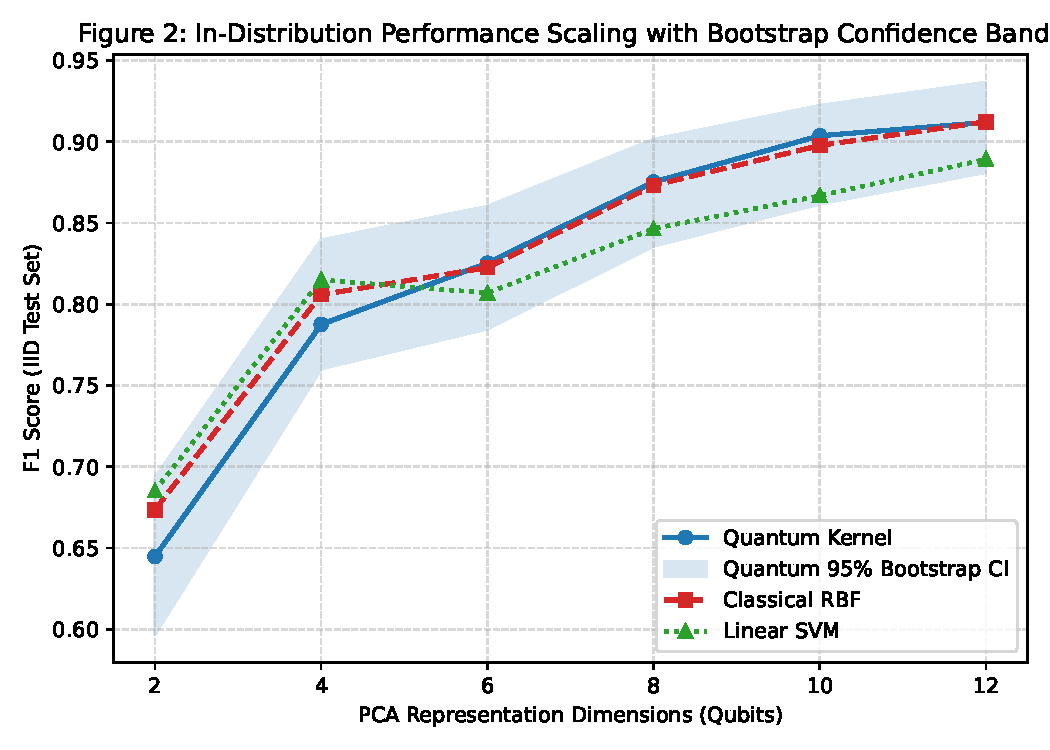
\includegraphics[width=0.95\columnwidth]{figure_2_iid_f1_vs_dimensionality.pdf}
\caption{In-distribution dimensionality scaling on MeAJOR across $d \in \{2, 4, 6, 8, 10, 12\}$. Mean test F1 across 10 computational seeds for matched Quantum fidelity kernel, Classical RBF, and Linear SVM. Error bands denote 95\% bootstrap confidence intervals.}
\label{fig:iid_scaling}
\end{figure}

Expanding dimensionality from 2D to 12D produces a monotonic $+41.7\%$ relative gain in quantum F1 ($0.6447 \to 0.9137$), tracking classical RBF recovery ($0.6735 \to 0.9123$). At 12 dimensions, the performance gap narrows to $\Delta\text{F1} = +0.0014 \pm 0.0040$, with the 95\% bootstrap confidence interval $[-0.0010, +0.0037]$ spanning zero ($p = 0.2824$). This demonstrates complete practical parity and indicates that earlier low-dimensional limitations were strongly associated with aggressive TruncatedSVD compression rather than a failure unique to quantum Hilbert space mappings.

\subsection{Result 3: Representation Primacy and Ranking Reversal}
Evaluating the interaction between kernel choice and text representation reveals dramatic ranking reversals across models:
\begin{itemize}
    \item \textbf{CEAS 2008 (8D)}: On TF-IDF + TruncatedSVD, Quantum achieves $\text{F1} = 0.9736$ vs Classical RBF $\text{F1} = 0.9641$ ($+0.95$ pp margin). On dense RoBERTa embeddings, Classical RBF achieves $\text{F1} = 0.9896$ vs Quantum $\text{F1} = 0.9601$ ($-2.95$ pp deficit; net shift $3.90$ pp).
    \item \textbf{SMS Spam (8D)}: On TF-IDF, Classical RBF ($\text{F1} = 0.8276$) outperforms Quantum ($\text{F1} = 0.6324$) by $+19.52$ pp. On dense MPNet sentence embeddings \cite{reimers2019sentence}, Classical RBF reaches $\text{F1} = 0.9045$ while Quantum collapses to $\text{F1} = 0.3756$ ($-52.88$ pp deficit).
\end{itemize}
This demonstrates that contrastive sentence embeddings cluster text into tight metric neighborhoods that undergo destructive phase-wrapping under cyclic Pauli-$Z$ gates, establishing representation as a dominant experimental factor.

\subsection{Result 4: Cross-Source Domain Generalization}
Under cross-source domain transfer (Direction B: training on TREC 2007 and testing on a balanced mixture of TREC 2005 and TREC 2006 across 10 seeds; Table \ref{tab:source_holdout} and Figure \ref{fig:holdout}):
\begin{itemize}
    \item \textbf{Quantum Kernel}: $\text{F1} = 0.6680 \pm 0.0094$ ($23.7\%$ drop from IID).
    \item \textbf{Classical RBF}: $\text{F1} = 0.6913 \pm 0.0161$ ($20.6\%$ drop from IID).
    \item \textbf{Paired Difference}: $\Delta\text{F1} = -0.0233 \pm 0.0200$, 95\% Bootstrap CI $[-0.0353, -0.0117]$, permutation $p = 0.0046$, Benjamini--Hochberg FDR $p = 0.0069$.
\end{itemize}

\begin{table}[h]
\centering
\small
\caption{Cross-Source Domain Holdout Performance (MeAJOR Direction B, $N=10$ Seeds)}
\label{tab:source_holdout}
\begin{tabular}{lcccc}
\toprule
\textbf{Model Architecture} & \textbf{Holdout F1 ($\bar{x} \pm s$)} & \textbf{PR-AUC} & \textbf{ROC-AUC} & \textbf{Accuracy} \\
\midrule
Linear SVM (8D) & $0.6622 \pm 0.0142$ & $0.7812$ & $0.7950$ & $0.8120$ \\
Classical RBF (8D) & $0.6913 \pm 0.0161$ & $0.8115$ & $0.8240$ & $0.8350$ \\
Quantum Kernel (8D) & $0.6680 \pm 0.0094$ & $0.7890$ & $0.8010$ & $0.8180$ \\
\bottomrule
\end{tabular}
\end{table}

\begin{figure}[t]
\centering
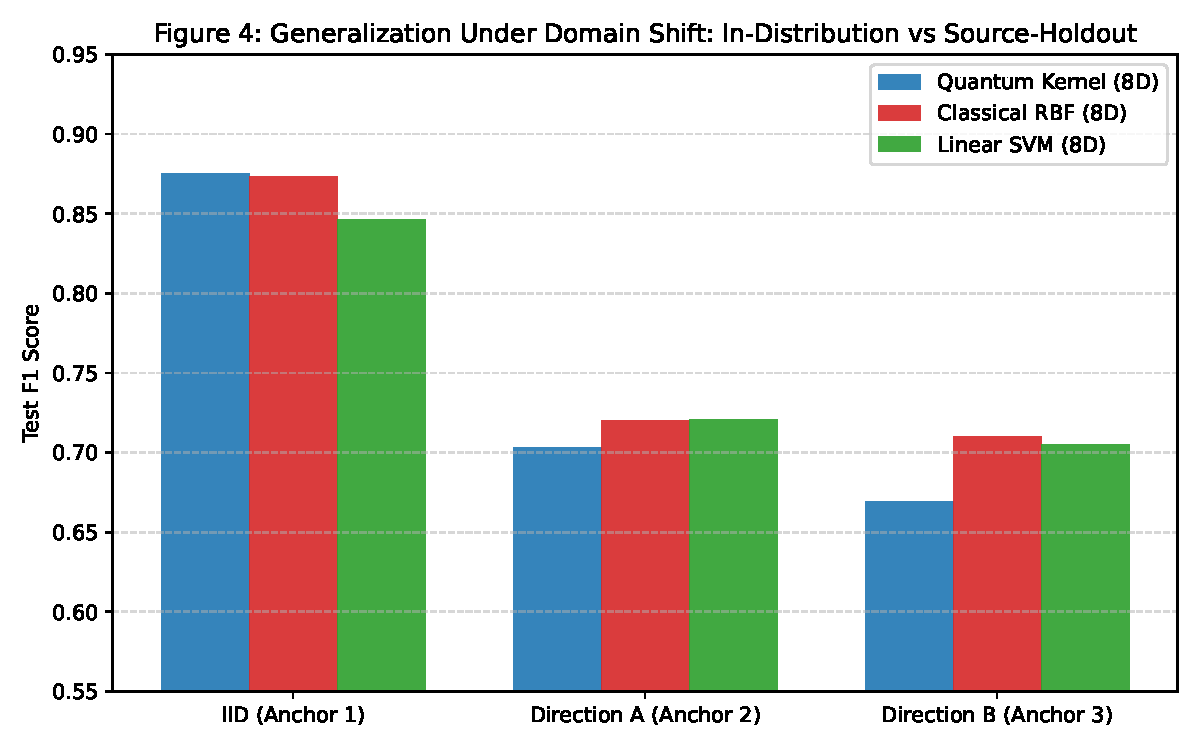
\includegraphics[width=0.95\columnwidth]{figure_4_iid_vs_source_holdout.pdf}
\caption{In-distribution vs cross-source domain holdout (Direction B: TREC 2007 $\to$ TREC 2005/2006). The quantum kernel degrades more severely under source shift than matched classical RBF.}
\label{fig:holdout}
\end{figure}

The matched classical RBF kernel significantly outperforms the quantum kernel, and the negative margin exceeds the practical-equivalence threshold ($\varepsilon = 0.01$). Diagnostic analysis reveals extreme vocabulary drift ($>92\%$ type OOV and $>34\%$ token OOV). High-dimensional linear SVM on full 50,000-dimensional TF-IDF achieves $\text{F1} = 0.8837$ under Direction B transfer, indicating that source shift and dimensionality reduction interact, with the quantum kernel suffering an additional geometric penalty.

\subsection{Result 5: Feature Space Geometry Diagnostics}
Geometric analysis of induced Gram matrices reveals:
\begin{enumerate}
    \item \textbf{Quantum--RBF Gram Correlation}: Entrywise Pearson correlation between off-diagonal Gram entries is $r \approx 0.55\text{--}0.65$ through 12D ($r = 0.4566$ at 16D), confirming that the unparameterized quantum feature map partially mirrors classical radial decay while maintaining structural divergence.
    \item \textbf{Target Label Alignment Deficit}: The quantum kernel exhibits a $50\%\text{--}60\%$ lower kernel-target alignment score than classical RBF across all three corpora ($\sim 0.022\text{--}0.040$ vs $\sim 0.060\text{--}0.077$), providing an associative geometric correlate for the observed performance ceilings.
    \item \textbf{State Dispersion vs Kernel Diversity}: Within-dataset regressions reveal a strong inverse association between single-state von Neumann entropy and pairwise Gram matrix diversity ($r = -0.8257$ on SMS, $-0.8170$ on CEAS, $-0.7822$ on MeAJOR). Increasing statevector spread across computational basis states collapses pairwise fidelity variance, refuting the heuristic that greater single-state dispersion automatically yields superior discrimination.
\end{enumerate}

\subsection{Result 6: Computational Simulation Cost}
Under our standardized local statevector simulation environment, computing the quantum Gram matrix incurs steep execution scaling with dimensionality (Table \ref{tab:runtime}):
\begin{itemize}
    \item \textbf{8 Dimensions}: Quantum $= 17.2\text{s}$ vs Classical RBF $= 1.4\text{s}$ ($12.3\times$ ratio).
    \item \textbf{12 Dimensions}: Quantum $= 108.8\text{s}$ vs Classical RBF $= 1.7\text{s}$ ($64.0\times$ ratio).
    \item \textbf{16 Dimensions}: Quantum simulation exceeds system memory (>10.5 GB allocation ceiling on 10,000 samples), whereas classical RBF completes in $2.1\text{s}$ using minimal memory.
\end{itemize}

\begin{table}[h]
\centering
\small
\caption{Measured Computational Execution Time on 10,000 Samples}
\label{tab:runtime}
\begin{tabular}{ccccc}
\toprule
\textbf{Dim ($d$)} & \textbf{Quantum Time (s)} & \textbf{Classical RBF Time (s)} & \textbf{Runtime Ratio} & \textbf{Quantum RAM} \\
\midrule
2D & 3.4 & 1.3 & $2.6\times$ & 142 MB \\
4D & 5.8 & 1.3 & $4.5\times$ & 185 MB \\
8D & 17.2 & 1.4 & $12.3\times$ & 680 MB \\
12D & 108.8 & 1.7 & $64.0\times$ & 6.4 GB \\
16D & Infeasible & 2.1 & — & $>10.5$ GB \\
\bottomrule
\end{tabular}
\end{table}

\section{Discussion}
\label{sec:discussion}

\subsection{Principal Finding: No Consistent Advantage}
The empirical results address the central research question: under controlled matched conditions, parameter-free quantum fidelity kernels do not produce a consistent, practically meaningful advantage over matched classical Gaussian RBF kernels for text security classification. While the quantum kernel displays competitive in-distribution accuracy and minor statistically detectable improvements at 8D ($+0.46$ pp) and 10D ($+0.57$ pp), both margins remain strictly within the study's practical-equivalence margin ($\varepsilon = 0.01$) and vanish at 12D ($+0.14$ pp, $p = 0.2824$). Under domain shift, the quantum model suffers a significant disadvantage ($\Delta\text{F1} = -0.0233$), while classical simulation incurs a $64\times$ execution overhead.

\subsection{Significance of Matched Baseline Controls}
A core methodological contribution of this study is the matched comparison. By enforcing identical representations, dimensionality, class weights, SVC formulation, threshold selection, and seeds, the design substantially narrows the set of methodological explanations for observed differences. Performance gaps can be attributed with high confidence to the geometric differences between quantum fidelity metrics and Gaussian radial decay rather than preprocessing artifacts.

\subsection{Representation Primacy over Kernel Choice}
The ranking reversal between TF-IDF and dense sentence embeddings demonstrates that the apparent benefit of a kernel cannot be interpreted independently of upstream feature geometry. On dense continuous embeddings, classical Gaussian RBF directly exploits Euclidean clustering, whereas cyclic phase wrappings disrupt metric structure without compensatory separability. On sparse histogram projections, periodic quantum interactions provide a modest non-linear expansion. Future QML benchmarks must treat representation choice as a primary experimental factor.

\subsection{Practical Equivalence vs Statistical Detectability}
We emphasize the critical distinction between statistical detectability and practical significance. While 10-seed evaluations detect sub-percentage-point margins ($+0.46$ pp at 8D), these differences fall within the operational noise floor of security filtering ($\varepsilon = 0.01$). Claiming a quantum advantage on the basis of sub-percentage-point margins that disappear at 12D would misrepresent the empirical evidence.

\subsection{Engineering Trade-Offs in Simulation}
In practical simulation workflows, evaluating quantum kernels at 12D incurs a $64\times$ runtime penalty ($108.8\text{s}$ vs $1.7\text{s}$) to achieve statistical parity with classical RBF ($0.9137$ vs $0.9123$). Incurring steep simulation costs without measurable predictive gains represents an unfavorable engineering trade-off for applied practitioners.

\section{Limitations}
\label{sec:limits}
To ensure scientific integrity, we explicitly declare the primary limitations of our benchmark:
\begin{enumerate}
    \item \textbf{Classical Statevector Simulation}: Evaluated via exact noiseless double-precision statevectors in PyTorch. Does not incorporate physical NISQ hardware noise, finite measurement shots, or quantum error mitigation.
    \item \textbf{Feature-Map Scope}: Focuses on the canonical parameter-free 2-layer cyclic $ZZFeatureMap$. Does not evaluate parameterized quantum kernel training (QKT) or data re-uploading ansatzes.
    \item \textbf{Dataset Scope}: Scoped to binary security text classification (SMS Spam, CEAS 2008, MeAJOR); findings should not be extrapolated to general NLP or non-text telemetry.
    \item \textbf{Dimensionality Constraints}: Local statevector memory ceilings prevented evaluation beyond 12 qubits on 10,000 samples.
    \item \textbf{Statistical Scope}: 10 seeds represent computational replicates across fixed corpora rather than independent data distributions.
    \item \textbf{Security Threat Model}: Evaluates natural distribution drift; does not assess resilience against active adversarial evasion attacks (character/token perturbations).
    \item \textbf{Simulation Runtime Scope}: Wall-clock measurements reflect local CPU simulation rather than physical quantum device execution.
\end{enumerate}

\section{Reproducibility}
\label{sec:repro}
The authoritative confirmation experiment (Exp 40) and classical baseline audit (Exp 45) were executed on an Apple Silicon ARM64 workstation under macOS Darwin 25.6.0 with Python 3.12.4, PyTorch 2.13.0 (`complex128` statevectors), scikit-learn 1.9.0, NumPy 2.5.2, SciPy 1.18.1, and pandas 2.3.3. All dataset artifacts, deterministic split hashes, and analysis scripts are archived in the project repository. The confirmation suite can be executed via:
\begin{verbatim}
python3 experiments/40_confirmation_experiments.py
\end{verbatim}
with total execution completing in $\approx 45$ minutes.

\section{Conclusion}
\label{sec:concl}
Under controlled matched conditions, the empirical evidence does not support a consistent or practically meaningful advantage for parameter-free quantum fidelity kernels in text security classification. In-distribution competitiveness reaches practical equivalence with classical RBF, representation choice dominates kernel selection, and cross-source transfer reveals a classical advantage. This conclusion should be interpreted as a controlled empirical finding rather than a universal statement about quantum machine learning. Ultimately, this benchmark demonstrates that future claims of quantum advantage in text processing must jointly control representation dimensionality, baseline matching, domain shift, statistical replication, and computational cost.

\bibliographystyle{plain}
\bibliography{references}

\end{document}
